\chapter{El arte de estimar}
\labch{estimadores-puntuales}

\begin{ideanote}
No podemos medir directamente los parámetros que nos interesan —como la media o la varianza poblacional— pero podemos estimarlos a partir de una muestra. ¿Qué distingue a un buen estimador de uno malo?
\end{ideanote}

Como ha venido quedando claro en el capítulo anterior, es un poco raro hablar de la media muestral, varianza muestral o proporción muestral \emph{si conocemos la media, varianza o proporción poblacional.} Sin embargo, básicamente estamos usando el mismo truco que cuando nos enseñaron por primera vez álgebra: usted tiene algo que no conoce, pero haga como que lo conoce y póngale por nombre \(x\).

Lo que haremos será intentar encontrar un buen\sidenote{para alguna definición de bueno} valor para los parámetros poblacionales a partir de una muestra. Teóricamente, podríamos usar cualquier receta que se nos ocurra. Podríamos decir que vamos a estimar la media tomando el promedio de los datos que salieron en orden impar, o que vamos a estimar la varianza elevando cada dato al cuadrado, sumando y dividiendo por \(n^3\). A veces una receta loca puede tener cierto sentido. Sin embargo, primero necesitamos definir cómo vamos a medir la calidad de un estimador. 

Un punto importante a tener en cuenta: ningún estimador es perfecto. Todos los estimadores dependen de la muestra y, por azar, podemos sacar justo la muestra en que todas las personas miden \qty{170}{\centi\meter} de una población cuyas estaturas se distribuyen normalmente, con media \qty{168}{\centi\meter} y desviación estándar \qty{5}{\centi\meter}. ¿Poco probable? Sí, pero no imposible. Un ejemplo menos extremo podría ser más claro, en que sacamos 4 personas que miden más de \qty{170}{\centi\meter} y una que mide \qty{168}{\centi\meter}. Sería difícil achuntarle a que la media poblacional es \num{168}. Además, incluso si resultara con esa muestra, usando la misma manera de estimar con otra muestra puede que dé otro valor. En resumen, un estimador puntual difícilmente nos dará el valor exacto del parámetro que estima, pero idealmente debería estar relativamente cercano para la mayoría de las muestras.

\begin{pausa}
Antes de ver cómo se evalúan los estimadores: ¿qué propiedades le gustaría que tuviera uno? Intente listar dos o tres características que le parezcan deseables.
\end{pausa}

Una forma de entender los estimadores es imaginar que son tiradores de dardos.

\resizebox{\linewidth}{!}{%
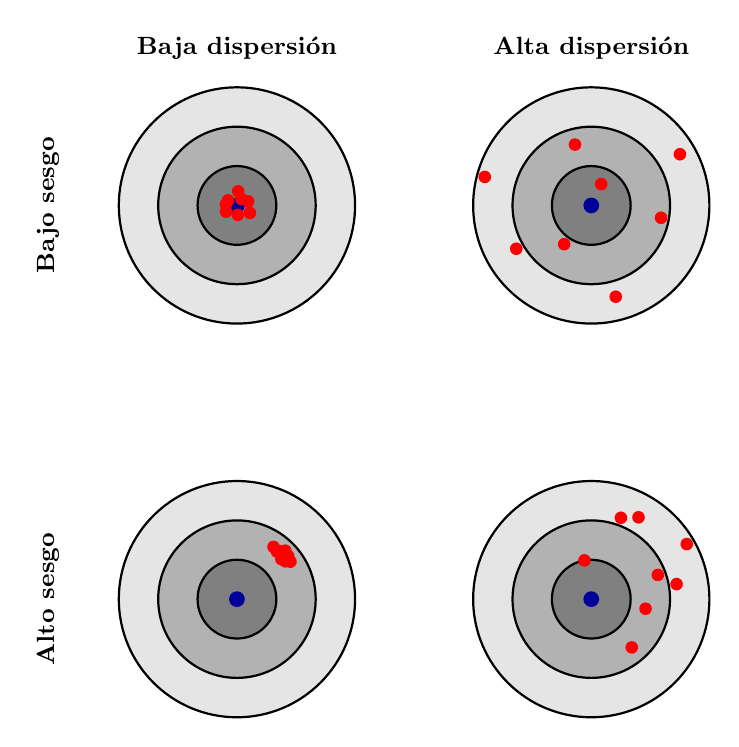
\begin{tikzpicture}
    % Column headers
    \node[font=\small\bfseries] at (0, 7.0) {Baja dispersión};
    \node[font=\small\bfseries] at (4.5, 7.0) {Alta dispersión};
    % Row headers
    \node[font=\small\bfseries, rotate=90] at (-2.4, 5) {Bajo sesgo};
    \node[font=\small\bfseries, rotate=90] at (-2.4, 0) {Alto sesgo};

    % Top-left: Bajo sesgo + Baja dispersión
    \begin{scope}[xshift=0cm, yshift=5cm]
        \fill[black!10] (0,0) circle (1.5);
        \fill[black!30] (0,0) circle (1);
        \fill[black!50] (0,0) circle (0.5);
        \draw[thick] (0,0) circle (1.5);
        \draw[thick] (0,0) circle (1);
        \draw[thick] (0,0) circle (0.5);
        \fill[blue!60!black] (0,0) circle (0.1);
        \fill[red] (20:0.15) circle (0.08);
        \fill[red] (85:0.18) circle (0.08);
        \fill[red] (150:0.13) circle (0.08);
        \fill[red] (210:0.16) circle (0.08);
        \fill[red] (275:0.12) circle (0.08);
        \fill[red] (330:0.19) circle (0.08);
        \fill[red] (55:0.10) circle (0.08);
        \fill[red] (175:0.14) circle (0.08);
    \end{scope}

    % Top-right: Bajo sesgo + Alta dispersión
    \begin{scope}[xshift=4.5cm, yshift=5cm]
        \fill[black!10] (0,0) circle (1.5);
        \fill[black!30] (0,0) circle (1);
        \fill[black!50] (0,0) circle (0.5);
        \draw[thick] (0,0) circle (1.5);
        \draw[thick] (0,0) circle (1);
        \draw[thick] (0,0) circle (0.5);
        \fill[blue!60!black] (0,0) circle (0.1);
        \fill[red] (30:1.3) circle (0.08);
        \fill[red] (105:0.8) circle (0.08);
        \fill[red] (165:1.4) circle (0.08);
        \fill[red] (235:0.6) circle (0.08);
        \fill[red] (285:1.2) circle (0.08);
        \fill[red] (350:0.9) circle (0.08);
        \fill[red] (65:0.3) circle (0.08);
        \fill[red] (210:1.1) circle (0.08);
    \end{scope}

    % Bottom-left: Alto sesgo + Baja dispersión
    \begin{scope}[xshift=0cm, yshift=0cm]
        \fill[black!10] (0,0) circle (1.5);
        \fill[black!30] (0,0) circle (1);
        \fill[black!50] (0,0) circle (0.5);
        \draw[thick] (0,0) circle (1.5);
        \draw[thick] (0,0) circle (1);
        \draw[thick] (0,0) circle (0.5);
        \fill[blue!60!black] (0,0) circle (0.1);
        \fill[red] (40:0.85) circle (0.08);
        \fill[red] (50:0.79) circle (0.08);
        \fill[red] (35:0.83) circle (0.08);
        \fill[red] (55:0.81) circle (0.08);
        \fill[red] (45:0.87) circle (0.08);
        \fill[red] (42:0.76) circle (0.08);
        \fill[red] (48:0.82) circle (0.08);
        \fill[red] (38:0.78) circle (0.08);
    \end{scope}

    % Bottom-right: Alto sesgo + Alta dispersión
    \begin{scope}[xshift=4.5cm, yshift=0cm]
        \fill[black!10] (0,0) circle (1.5);
        \fill[black!30] (0,0) circle (1);
        \fill[black!50] (0,0) circle (0.5);
        \draw[thick] (0,0) circle (1.5);
        \draw[thick] (0,0) circle (1);
        \draw[thick] (0,0) circle (0.5);
        \fill[blue!60!black] (0,0) circle (0.1);
        \fill[red] (70:1.1) circle (0.08);
        \fill[red] (20:0.9) circle (0.08);
        \fill[red] (350:0.7) circle (0.08);
        \fill[red] (100:0.5) circle (0.08);
        \fill[red] (30:1.4) circle (0.08);
        \fill[red] (310:0.8) circle (0.08);
        \fill[red] (60:1.2) circle (0.08);
        \fill[red] (10:1.1) circle (0.08);
    \end{scope}
\end{tikzpicture}%
}


Cada tirador está tratando de dar en el blanco. Sin embargo, hay varias formas en que se puede fallar y sólo una en que se puede ser perfectamente exitoso \emph{siempre.} En nuestro caso, un estimador está tratando de dar en el blanco. El blanco es algún parámetro de nuestra población. Generalmente, consideraremos la media o varianza, pero podría ser cualquier cosa: mediana, curtosis, simetría, etc. Nuestro ideal sería encontrar un estimador que
\begin{enumerate}
\item En general esté cerca del parámetro. Es imposible que siempre esté cerca, pero ojalá la mayor parte de las veces.
\item En general no sea muy disperso. Es imposible que no tenga dispersión, pero si esa dispersión es de alguna forma pequeña, sirve.
\end{enumerate}

¿Por qué es imposible pedir el estimador perfecto? Un estimador es un cálculo que se puede hacer para todas las muestras posibles. Eso quiere decir que, incluso en el mejor de los estimadores posibles, podríamos tener una situación como la del gráfico\\
\begin{tikzpicture}
    \begin{axis}[
        width=10cm,
        height=6cm,
        axis lines=middle,
        xlabel={$x$},
        ylabel={$f(x)$},
        domain=-4:4,
        samples=100,
        ymin=0,
        enlargelimits=false,
        clip=false,
        hide y axis,
        xtick=\empty
        ]
        \addplot[blue!80!black, thick] {exp(-x^2/2)/sqrt(2*pi)};
        \draw[thin, gray] (axis cs:0,0) -- (axis cs:0,0.4);
        \node[below] at (axis cs:0,0) {$\mu$};
        \draw[thin, gray] (axis cs:-2.025, 0) -- (axis cs:-2.025, 0.05);
        \node[below] at (axis cs: -2.025, 0) {$\mean{x}$};
        \fill[red] (axis cs:-1,0) circle (2pt);
        \fill[red] (axis cs:-1.3,0) circle (2pt);
        \fill[red] (axis cs:-2.3,0) circle (2pt);
        \fill[red] (axis cs:-3.5,0) circle (2pt);
        \end{axis}
\end{tikzpicture}
donde el estimador \(\mean{x}\), aplicado a esa muestra, no da cerca del parámetro \(\mu\).

Nuestro plan será
\begin{enumerate}
\item Definir qué hace que un estimador sea bueno.
\item Definir estrategias razonables para encontrar estimadores.
\end{enumerate}

Antes de seguir, definamos qué es un estimador.

\begin{definition}
\labdef{estimador}

Un estimador \(\estim{\theta}\) del parámetro poblacional \(\theta\) es una función de la muestra \[\estim{\theta} = f(X_1, X_2,\ldots, X_n)\]

\end{definition}

\section{¿Qué hace que un estimador sea bueno? Error cuadrático medio y amigos}
\labsec{ECM}

Si \(\estim{\theta}\) es un estimador de un parámetro \(\theta\), ambos son cosas distintas. Por un lado \(\theta\) es un número que calculamos a partir de la \emph{población} y, por lo tanto, es fijo.\sidenote{la población \emph{no} cambia} Por otra parte, \(\estim{\theta}\) es un número distinto para cada muestra y, como la muestra se supone aleatoria, eso significa que un estimador es una variable aleatoria. Esto tiene como consecuencia que un estimador tiene todas las cosas que una variable aleatoria tiene, como una distribución de probabilidad, esperanza, varianza, etc.

Para este estimador, podemos calcular la diferencia entre el valor que dio para una muestra y el valor que quiere estimar \[\estim{\theta} - \theta\] pero igual es mala idea así, porque si para una muestra nos da un valor y para otra nos da justo el opuesto, cuando juntemos a través de todas las muestras, capaz que nos dé injustificadamente \(0\). Usemos la técnica que hemos usado a través del curso y elevemos al cuadrado \[\left(\estim{\theta} - \theta\right)^2.\]

¿Cómo juntamos el \enquote{a través de todas las muestras} que aparece mencionado en el párrafo anterior como si fuera tan fácil? Bueno, no es difícil. ¿Qué tal esto? \[\esp{\left(\estim{\theta} - \theta\right)^2}\] Precisamente lo que queremos: el valor esperado de las diferencias, pero al cuadrado para evadir los problemas de signo.

\formal
Definiremos como el \emph{error cuadrático medio} de un estimador \(\estim{\theta}\) de un parámetro \(\theta\) al valor \[\ecm\left( \estim{\theta} \right) = \esp{\left(\estim{\theta} - \theta\right)^2}\]

\informal
El ECM es poco práctico de esa manera, pero además no nos dice mucho (más allá de que parezca razonable). Hay una manera en que podemos calcularlo más fácilmente y además tiene una interpretación transparente.

\begin{align*}
\ecm\left( \estim{\theta} \right) &= \esp{\left(\estim{\theta} - \theta\right)^2}\\
&= \esp{\estim{\theta}^2 -2\estim{\theta}\theta + \theta^2}
\intertext{\(\theta\) es un número}
&= \esp{\estim{\theta}^2} -2\theta\esp{\estim{\theta}} + \theta^2  
\intertext{por otra parte, despejando \(\esp{\estim{\theta}^2}\) de \(\var{\estim{\theta}} = \esp{\estim{\theta}^2} - \esp{\estim{\theta}}^2\)}
&= \var{\estim{\theta}} + \esp{\estim{\theta}}^2 - 2\theta\esp{\estim{\theta}} + \theta^2 
\intertext{pero los tres últimos términos hacen un cuadrado de binomio}
\ecm\left( \estim{\theta} \right)&= \var{\estim{\theta}} + \left( \esp{\estim{\theta}} - \theta \right)^2
\end{align*}

Esta forma del ECM es más práctica pero además nos muestra que el error cuadrático medio está compuesto de dos partes: la varianza del estimador y la diferencia entre el valor esperado del estimador y el verdadero valor del parámetro. 

Definiremos \[B\left(\estim{\theta}\right) = \esp{\estim{\theta}} - \theta\] como el \emph{sesgo} de \(\estim{\theta}\).  Idealmente, un estimador debería tener sesgo \(0\), es decir, la esperanza del estimador debería ser el parámetro que estima. Cuando esto ocurre, se dice que el estimador es \emph{insesgado.}\sidenote{en otras palabras, el sesgo mide el error que \emph{sistemáticamente} comete nuestro estimador en promedio.}

La varianza del estimador, por otra parte, se considera como su \emph{eficiencia.} El estimador \(\estim{\theta}_1\) es más eficiente que el estimador \(\estim{\theta}_2\) si \[\var{\estim{\theta}_1}< \var{\estim{\theta}_2}.\] Mientras más eficiente un estimador, sus estimaciones estarán más concentradas. \emph{Adonde} estén concentradas tiene que ver con el sesgo del estimador.

\subsection{Cota de Cramér-Rao}

El estimador perfecto sería insesgado y con varianza \(0\). Ese estimador no existe.

Hay una cota inferior de las varianzas de los posibles estimadores: la cota de Cramér-Rao. 